\section{Polarization}

\begin{definition}{Polarization Basis}
  Well-defined (complex) unit vector distribution tangential to far-field sphere (unit normal $\bs{n}$).
\end{definition}

\begin{equation*}
  \bs{e}_{\text{cr}}(\vartheta,\varphi) = \bs{n}(\vartheta,\varphi) \times \bs{e}_{\text{co}}^{*}(\vartheta, \varphi)
\end{equation*}

$\bs{C}(\vartheta,\varphi)$ can be decomposed into components:

\begin{align*}
  &\bs{C}(\vartheta,\varphi) = C_{\text{co}}\bs{e}_{\text{co}} + C_{\text{cr}}\bs{e}_{\text{cr}},\\
  &C_{\text{co/cr}} = \bs{C}(\vartheta,\varphi) \cdot \bs{e}_{\text{co/cr}}^{*}(\vartheta,\varphi).
\end{align*}

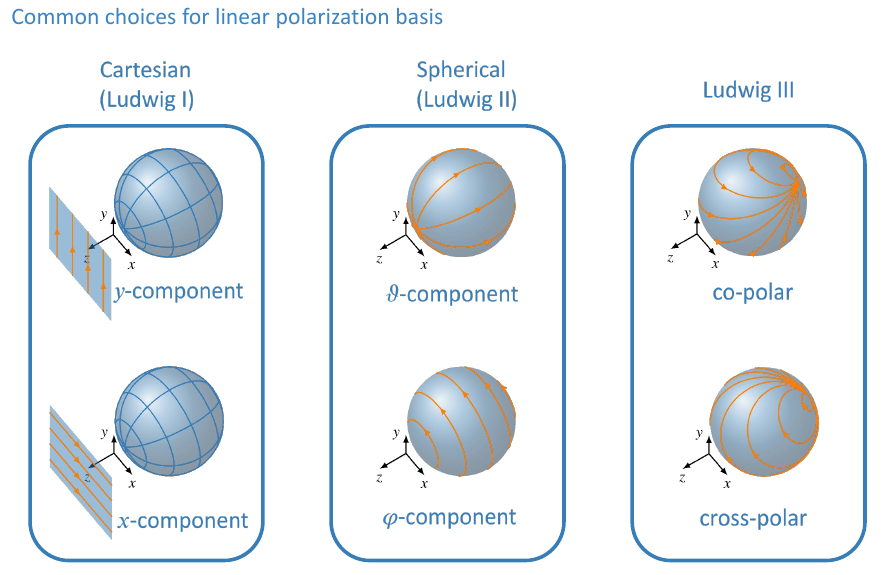
\includegraphics[angle=90, height=7cm]{content/at_meas/pictures/linear_polarization_bases}

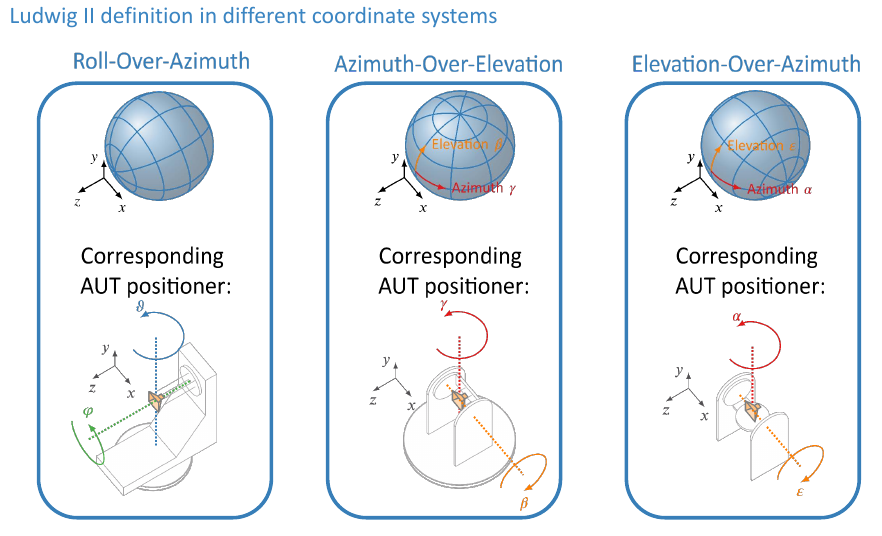
\includegraphics[angle=90, height=7cm]{content/at_meas/pictures/ludwig_II}

\subsection{Conversion between Linear Polarization Bases}


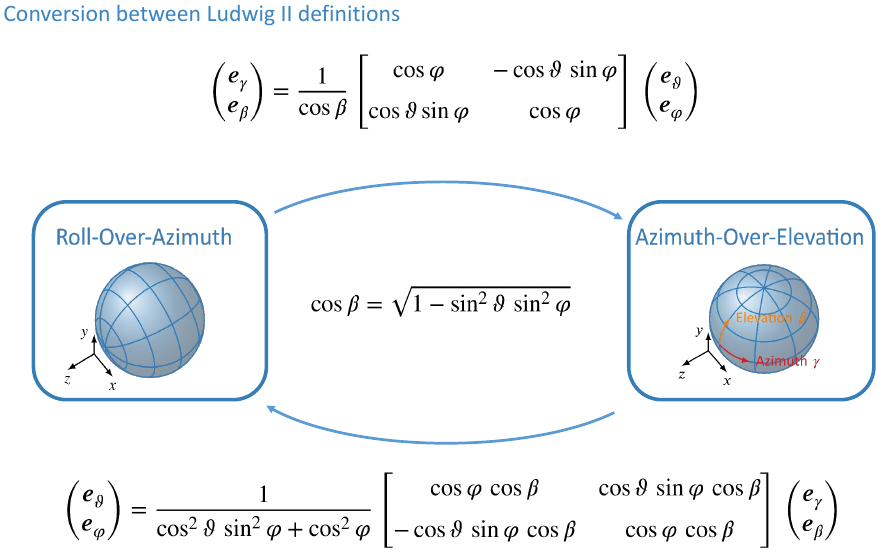
\includegraphics[width=8.5cm]{content/at_meas/pictures/ludwig_II_conversion1}
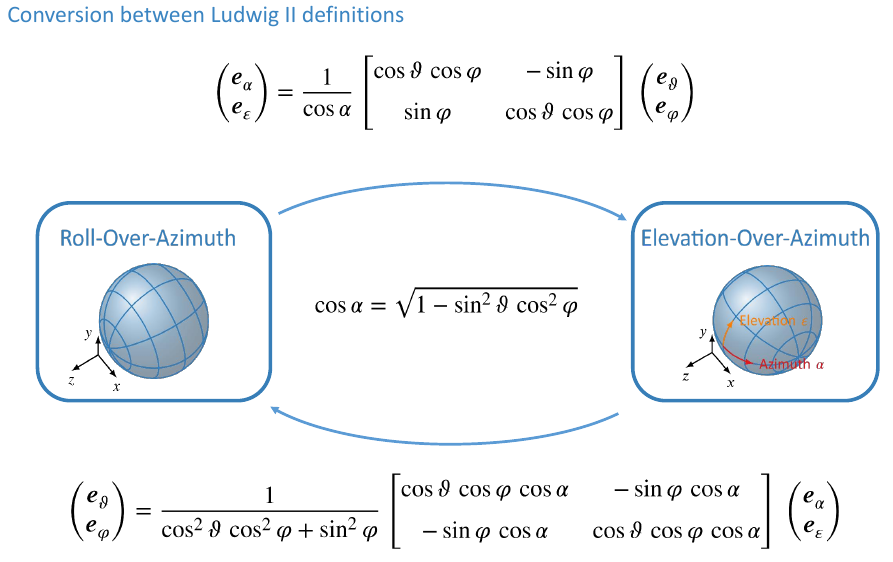
\includegraphics[width=8.5cm]{content/at_meas/pictures/ludwig_II_conversion2}

Conversion between Ludwig II and Ludwig III basis:

\begin{equation*}
  \begin{pmatrix}
    \bs{e}_{\text{co,3L}}\\
    \bs{e}_{\text{cr,3L}}
  \end{pmatrix}
  =
  \begin{bmatrix}
    \cos(\varphi - \varphi_{0}) & - \sin(\varphi - \varphi_{0})\\
    \sin(\varphi - \varphi_{0}) & \cos(\varphi - \varphi_{0})
  \end{bmatrix}
  \begin{pmatrix}
    \bs{e}_{\vartheta}\\
    \bs{e}_{\varphi}
  \end{pmatrix}
\end{equation*}

\begin{equation*}
  \begin{pmatrix}
    \bs{e}_{\vartheta}\\
    \bs{e}_{\varphi}
  \end{pmatrix}
  =
  \begin{bmatrix}
    \cos(\varphi - \varphi_{0}) & \sin(\varphi - \varphi_{0})\\
    - \sin(\varphi - \varphi_{0}) & \cos(\varphi - \varphi_{0})
  \end{bmatrix}
  \begin{pmatrix}
    \bs{e}_{\text{co,3L}}\\
    \bs{e}_{\text{cr,3L}}
  \end{pmatrix}
\end{equation*}

$\varphi_{0} = 0 \implies \bs{e}_{\text{co,3L}} = \bs{e}_{x}$ in main radiation direction ($\bs{e}_{z}$).

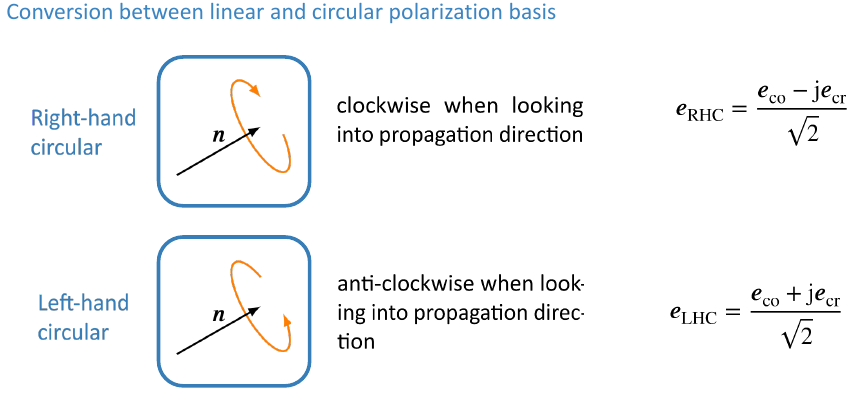
\includegraphics[width=7.5cm]{content/at_meas/pictures/linear_and_circular_polarization_conversion}

\subsection{Elliptical Polarization}

The most general case.\\
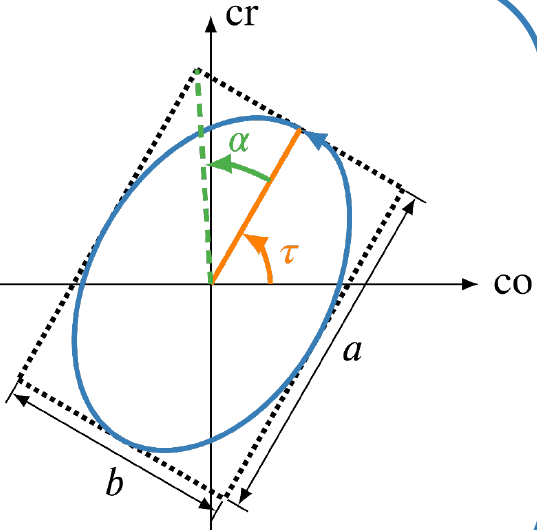
\includegraphics[width=3cm]{content/at_meas/pictures/elliptical_polarization}\\
\begin{itemize}
    \item Tilt angle
    \begin{equation*}
      \tau = \dfrac{\angle(C_{\text{LHC}}) - \angle(C_{\text{RHC}})}{2} = -\dfrac{\delta_{c}}{2}
    \end{equation*}
   \item Axial Ratio
   \begin{equation*}
     r = \dfrac{a}{b} = \dfrac{1}{\tan \alpha} = \dfrac{|C_{\text{RHC}}| + |C_{\text{LHC}}|}{|C_{\text{RHC}}| - |C_{\text{LHC}}|} = \dfrac{|\rho_{C}| + 1}{|\rho_{C}| - 1}
   \end{equation*}
  $r = \infty$ $\implies$ linear\\
  $r = 1$ $\implies$ circular\\
  $1 < r < \infty$ $\implies$ elliptical\\
  $\rho_{C} = \dfrac{C_{\text{RHC}}}{C_{\text{LHC}}}, \quad \delta_{C} = \angle(\rho_{C})$
\end{itemize}


\subsection{Poincaré Sphere}

\begin{center}
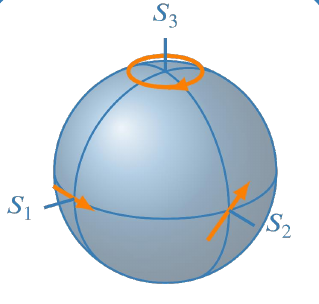
\includegraphics[width=5cm]{content/at_meas/pictures/poincare_sphere}
\end{center}

Stokes Parameters:

\begin{align*}
  &S_{0} = {|E_{co}|}^{2} + {|E_{cr}|}^{2} = {|E_{\text{LHC}}|}^{2} + {|E_{\text{RHC}}|}^{2}\\
  &S_{1} = {|E_{co}|}^{2} - {|E_{cr}|}^{2}\\
  &S_{2} = {|E_{45°}|}^{2} - {|E_{135°}|}^{2}\\
  &S_{3} = {|E_{\text{LHC}}|}^{2} - {|E_{\text{RHC}}|}^{2}\\
\end{align*}

\begin{align*}
  p = \dfrac{\sqrt{S_{1}^{2} + S_{2}^{2} + S_{3}^{2}}}{S_{0}}: \quad \text{degree of polarization}
\end{align*}
